\chapter{Microbial population structure and genetic heterogeneity in a hypersaline environment}

\section{Abstract}

\section{Introduction}

The increasing number of microbial genomes sequenced over the last years, driven by the higher-throughput and lower cost of sequencing technologies, has pushed the field of comparative genomics, allowing for comparisons of the genomes of organisms from the same genus and even closely related strains \cite{Fricke:2011gy,Doroghazi:2013gf,Grad:2013tc,Reno:2009bq}, in search of insights into their evolutionary history and environmental adaptation \cite{Reno:2009bq,ZhuofeiXu:2011fp}. This has been a particularly powerful approach in medical microbiology, where multiple cultivated strains are available, allowing for a deep coverage of microbial species of medical interest \cite{Feero:2011fr}. Some of this has been replicated in microorganisms isolated from the environment (non-clinical settings), including members of the \textit{Vibrio} genus \cite{Cordero:2012ik} and \textit{Sulfolobus} \cite{Reno:2009bq}.
 
The development of culture-independent approaches, has allowed to remove some of the restrictions of culture-based comparative genomics, by allowing us to capture directly the taxonomic, functional and genetic diversity of the members of microbial community, by direct sequencing of their DNA \cite{Bragg:2014kv}. The main challenge in metagenomic studies, is given by the complexity of some microbial communities, allowing only to capture a glimpse of the taxonomical and functional diversity, and not providing enough information to explore the genetic diversity that is present. 

In the case of low to moderate microbial communities (~2-30 dominant microbial species), using the appropriate sequencing technologies and sampling approaches, it is possible to reconstruct the genomes for some of the dominant members of the community \cite{Bragg:2014kv}. But in reality, these genomes do not represent a single clone, but are a composite of multiple related strains \cite{Podell:2013kx,Allen:2005dg}, where this fine-scale genetic variation could have functional relevance for the members of the community \cite{Lo:2007ht,Hemme:2010ds,Palenik:2009kx}.

Several studies have approached the study of microbial communities with the goal of quantifying the level of fine-scale genetic variation present in its members \cite{Wilmes:2009bn}, by using metagenomic approaches. These studies can be divided in two groups, based on the type of reference used to quantify genetic heterogeneity. A first group, approached a natural microbial community, obtained metagenomic sequence from the system, and then used reference genomes from isolates to quantify the genetic variation present in the microbial community. Examples of this approach include the study of \textit{Synechococcus} coastal populations \cite{Tai:2011jo} and in the human gut microbiome \cite{Schloissnig:2012hx}. The limitation of this type of studies, is that not necessarily the reference genomes used are derived from the same environment as the metagenomic sample. In addition, it is possible to miss novel and abundant groups, by just focusing on the genomes that are available through isolates \cite{Podell:2013kx,Herlemann:uy}. A second type of approach, is to use assembly-based metagenomics, which allows to recover a set of habitat-specific genomes, on which the genetic heterogeneity present in the community can be quantified. Although this approach provides a more complete and less biased picture of the genetic diversity, it is limited to communities with low species diversity, such as acid mine drainage \cite{Allen:2007ju} or heavy-metal contaminated sites \cite{Hemme:2010ds}.

The metagenomic studies carried out on the Lake Tyrrell microbial community, allowed us to assembled 15 Archaeal genomes and 1 Bacterial \cite{Narasingarao:2012kp,Podell:2013kx,Podell:2013fp}, providing a set of habitat-specific genomes that can be used to study fine-scale genetic variability within this community.

Microscale genetic heterogeneity has been previously studied in hypersaline ecosystems, via comparative genomics, such as in the case of \textit{Salinibacter ruber} \cite{PeNtildeA:2010ie}, or using metagenomic approaches \cite{Legault:2006kh,Pasic:2009bo,}. In both cases, this has been done using reference genomes from isolates, not necessarily recovered from the sample place where the metagenomic sampling was performed. 

In this chapter we study the fine-scale genetic diversity present in the Laker Tyrell microbial community, by combining a deep-sequencing metagenomic approach, with the availability of a set of habitat-specific genomes. In addition, we looked at two different temporal samples, collected in two different seasons, which can provides us with insights on the stability (both in abundances and in population structure) of this community over time.


\section{Material and Methods}

\subsection{Sample Collection and Sequencing}
Surface water samples from Lake Tyrrell were collected in 2007, during two different seasons, summer (January) and winter (August), with two days of difference in each season (January 23 \& 25, August 7 \& 9). Each water sample was filtered directly into a Sterivex cartridge (Milipore, Bedford, MA, USA) (\SI{0.22}{\micro\meter}) using a peristaltic pump. For DNA extraction, each Sterivex was processed according to the following protocol:

\begin{itemize}
\item Addition of Proteinase K to a final concentration of 0.5 mg/ml\textsuperscript{-1} and SDS to a final concentration of 1\%.
\item Incubation at 55\textsuperscript{o}C for 25 minutes, followed by incubation at 70\textsuperscript{o}C for 5 minutes.
\item Transfer of the lysate from the Sterivex to a clean Eppendorf tube.
\item Nucleic acid extraction with two steps of phenol-chloroform extraction. 
\end{itemize}

For all four samples, construction of the sequencing libraries was done at the UC San Diego IGM Genomics Center. The libraries were multiplexed and sequenced on a single lane of Illumina HiSeq (Illumina, San Diego, CA), using the high-throughput mode, with pair-ended reads of 100 nucleotides in length.

The demultiplexed reads were processed using Nesoni 0.117 (\url{http://www.vicbioinformatics.com/software.nesoni.shtml}) to remove adapters, trim low quality positions, and remove low-quality reads from the datasets. For trimming, a minimum quality score of 20 was used, and all reads shorter than 70 nucleotides (after trimming) were removed.

\subsection{Read Mapping}

The trimmed reads were mapped against a set of habitat-specific genomes (Table \ref{GenomeTable} generated by the assembly of metagenomic information of the Lake Tyrrell microbial community \cite{Narasingarao:2012kp,Podell:2013kx,Podell:2013fp}. In addition, an archaeal isolate, \textit{Candidatus} Halobonum tyrrellensis \cite{Ugalde:2013hb}, obtained from samples collected in August of 2007, was included in this set of reference genomes. Each library (January 23, January 25, August 7 and August 9) was mapped independently to the reference genomes, using Bowtie 2.2.1 \cite{Langmead:2012jh} with the \textit{very-sensitive} alignment option and adjusting the N-ceiling function to (0,0.01) to reduce the number of ambiguous characters present in the alignment. Several tools were used for the analysis of the resulting files, including SAMtools 0.1.19\cite{Li:2009ka}, BEDtools 2.17 \cite{Quinlan:2010km}, and BCFtools 0.2.0 (\url{http://samtools.github.io/bcftools/bcftools.html}).

Coverage plots were generated with custom Python scripts, using the BAM files generated by read mapping.

To determine the differential coverage of each gene in the reference genomes, we used the RPKM calculation (reads per kilobase per million reads mapped), stated in the following equation:

\begin{center}
\scalebox{1.2}{
\(
\text{RPKM} = \frac{\text{\textnumero{} of mapped reads to the gene} * \num{e9}}{\text{\textnumero{} of reads mapped in the experiment} * \text{Gene length}}
\)
}
\end{center}

To facilitate the visualization of differences between samples from January and August using the RPKM values, these were normalized using this formula:

\begin{center}
\scalebox{1.2}{
\(
\log_{2}(\frac{\text{January RPKM}}{\text{August RPKM}})
\)
}
\end{center}

A two-tailed Fisher exact test (pvalue $<$ 0.05) was used to determine which genes had differential recruitment of reads between the two seasons (January and August). A complete list of these genes in each of the genomes can be found here (XXX).

\subsection{Taxonomic Classification of Mapped and Unmapped Reads}

To compare the taxonomic diversity found in the mapped and unmapped reads, both sets were classified using Phylosift 1.0.1 \cite{Darling:2014ej}, with the provided set of marker genes. These markers included all of the January 2007 genomes that were assembled previously from the Lake Tyrrell community \cite{Narasingarao:2012kp,Podell:2013kx} (all the genomes with the prefix J07 in Table \ref{GenomeTable}), but did not include the more recent ones, recently assembled from metagenomic samples from the August 2007 community, and described in \cite{Podell:2013fp}.

\subsection{Variation Analysis}

The resulting BAM files with the information for the mapped reads were processed with Picard Tools 1.99 (\url{http://picard.sourceforge.net}), to sort and reorder the mapping information. GATK 2.7.2 (\cite{DePristo:2011fo} was used to realign indel regions found by mapping against the reference genomes. These corrected files were processed using Freebayes v9.9.2-29-g9ed353c \cite{Garrison:2012wb} (ploidy:1, minimum base quality: 20, minimum mapping quality: 30) to obtain a set of high-quality variations. Quantification of the type of variations (in particular within the category of single nucleotide polymorphisms, or SNPs) was done using SnpEff \cite{Cingolani:2012cz} and visualized using custom developed Python scripts. 

To calculate the role of selective pressure in each gene, we calculated the ratio of non-synonymous to synonymous polymorphisms. Commonly this ratio is referred as dN/dS, but in this context we are looking at populations (we are not able to distinguish individual members of the population), so it will be referred as pN/pS \cite{Schloissnig:2012hx}. Calculation of the pN/pS values for each coding sequence was done using custom Python scripts, based on the approach used in Tai \textit{et al.} \cite{Tai:2011jo}. For each gene, the pN/pS value was calculated as:

\begin{center}
\scalebox{1.6}{
\(
\frac{\text{pN}}{\text{pS}} = \frac{\frac{\text{Observed non synonymous mutations}}{\text{Number of non synonymous sites}}}{\frac{\text{Observed synonymous mutations}}{\text{Number of synonymous sites}}}
\)
}
\end{center}

All of the visualizations of these results were done using custom Python scripts. To evaluate the differences in functional classifications, we used the Cluster of Orthologuous Groups (COGs) \cite{Tatusov:2003fk} annotation of each gene. Comparisons of abundance were done using an odds ratio test calculated as:

\begin{center}
\scalebox{1.6}{
\(
\frac{\frac{\text{\textnumero{} of proteins under selection in category X}}{\text{\textnumero{} of proteins not under selection in category X}}}{\frac{\text{Total \textnumero{} of proteins under selection, minus category X}}{\text{Total \textnumero{} of proteins not under selection, minus category X}}}
\)
}
\end{center}

Statistical significance was evaluated using the 2X2 contingency table with a one-tailed Fisher exact test (pvalue $<$ 0.05).


\subsection{Statistical and Computer analysis}

All the analyses were carried out on a large cluster instance (c3.8xlarge: 32 Intel Xeon E5-2680 v2 cores, 60 Gb RAM) using the Elastic Cloud Computing (EC2) infraestructure from Amazon Web Services (AWS). Plotting and calculations were carried out using custom developed Python scripts, using the standard packages and the libraries Biopython \cite{Cock:2009hj}, Numpy \cite{Oliphant:2007ud} , Pandas \cite{mckinney-proc-scipy-2010}, PyCogent \cite{Knight:2007gp} and Matplotlib \cite{Hunter:2007ih}. All statistical analysis were carried out using Python scripts and the Scipy libraries \cite{Oliphant:2007ud}. IPython notebooks \cite{Perez:2007wf} and scripts are available on a repository on Github (XXX).


\begin{table}[!htdp]
\small
\caption{List of the Lake Tyrrell habitat-specific genomes used for read mapping}
\begin{center}
\resizebox{\textwidth}{!}{%
\begin{tabularx}{\textwidth}{L{5cm}R{2cm}R{1.4cm}p{2cm}p{1cm}}
\hline
\textbf{Genome name (abbrv)} & \textbf{Length} & \textbf{G+C pct} & \textbf{\textnumero{} scaffolds} & \textbf{Reference} \\
\hline
\textit{Haloquadratum walsbyi} J0HQW1 & 3,549,539 & 47 & 1 & \cite{Podell:2013kx} \\
\textit{Haloquadratum walsbyi} J0HQW2 & 3,475,501 & 49 & 1 & \cite{Podell:2013kx} \\
\textit{Haloquadratum} sp. J07HQX50 & 3,019,909 & 50 & 2 & \cite{Podell:2013kx} \\
\textit{Nanosalinarum} sp. J07AB56 & 1,215,802 & 56 & 3 & \cite{Narasingarao:2012kp} \\
\textit{Nanosalinarum} sp. J07AB43 & 1,277,157 & 43 & 7 & \cite{Narasingarao:2012kp} \\
\textit{Halonotius} sp. J07HN4 & 2,888,659 & 61 & 2 & \cite{Podell:2013kx} \\
\textit{Halonotius} sp. J07HN6 & 2,529,000 & 63 & 6 & \cite{Podell:2013kx} \\
uncultured archaeon sp. J07HX64 & 2,982,938 & 64 & 1 & \cite{Podell:2013kx} \\
uncultured archaeon sp. J07HX5 & 2,040,945 & 60 & 1 & \cite{Podell:2013kx} \\
\textit{Halobaculum} sp. J07HB67 & 2,649,547 & 67 & 3 & \cite{Podell:2013kx} \\
\textit{Halorubrum} sp. J07HR59 & 2,120,805 & 59 & 7 & \cite{Podell:2013kx} \\
\textit{Salinibacter} sp. J07SB67 & 1,931,021 & 67 & 443 & \cite{Podell:2013kx} \\
\textit{Halorubrum} sp. A07HR60 & 2,876,249 & 59 & 14 & \cite{Podell:2013fp} \\
\textit{Halonotius} sp. A07HN63 & 2,392,686 & 63 & 37 & \cite{Podell:2013fp} \\
\textit{Halorubrum} sp. A07HR67 & 2,890,468 & 67 & 16 & \cite{Podell:2013fp} \\
uncultured archaeon A07HB70 & 2,389,822 & 71 & 15 & \cite{Podell:2013fp} \\
\textit{Candidatus} Halobonum tyrellensis G22 & 3,675,087 & 70 & 72 & \cite{Ugalde:2013hb} \\
\hline

\end{tabularx}
}
\end{center}
\label{GenomeTable}
\end{table}


%%%%%%%%%%
\clearpage
\section{Results and Discussion}

\subsection{Overview of the Illumina datasets}

In all four samples, between 71\% to 74\% of the original reads were retained after trimming and quality filtering (Table \ref{LibSequenceQC}), representing in average ~6.9 billion bases per sample.

Preliminary visualization of the community composition was done by looking at the G+C content of each of the libraries. This allows to capture broader differences in community composition between the samples \cite{Podell:2013kx,Ghai:2012fb,Podell:2013fp}. Figure \ref{ReadsGCplot} shows the differences between the four libraries, highlighting the location of the reference genomes that will be used for read mapping, and where recovered from this same community. The plot shows that the January community (in particular the sample collected on January 25) is dominated by organisms with a low G+C content, compared to the August community. This is similar to previous observations for the Lake Tyrrell microbial community \cite{Podell:2013fp}. The main driver of these differences was suggested to be the ionic composition of the water column, in particular the concentration of magnesium, which is higher in the January samples compared to the August ones (Table \ref{LT_chemical}), and where microorganisms like \textit{Haloquadratum} (J07HQW1, J07HQW2 and J07HQX50) are more abundant in the January sample due to their tolerance to higher concentrations of magnesium \cite{Podell:2013fp}. 

Besides the differences between different months among the samples, we can observe differences within the January libraries, with different G+C peaks in the January 23 versus the January 25 sample. In particular, the January 25 sample shows a higher peak at lower G+C, compared to the January 23 sample. Looking back into the chemical measurements done for these samples (\ref{LT_chemica}) \cite{Podell:2013fp}, we can see that the magnesium concentrations on the January 23 sample are lower compared to January 25. Weather records showed that there was an input of freshwater due to a storm previous to the sampling on January 23 \cite{Podell:2013fp}, which suggests an effect on the overall concentrations of dissolved salts, including magnesium. After two days, mainly due to water evaporation, the concentration of dissolved salts in the water column increased, which could explain the difference in the G+C plots, and therefore the changes in population abundances between the different samples. 



%Table, Summary libraries
\begin{table}[hbt]
  \caption{Summary of the total reads before and after trimming, for each of the four Illumina HiSeq libraries.}
  \begin{tabularx}{\textwidth}{L{2.2cm}R{2cm}R{3cm}R{3.2cm}R{2cm}}
  \hline
    \textbf{Library name} & \textbf{Total reads} & \textbf{Read-pairs after QC} & \textbf{Unpaired reads after QC} & \textbf{Total bases (Gb)} \\
    \hline 
    \textit{January 23} & 49,963,357 & 37,016,243 & 7,679,004 & 7,978.18\\
    \textit{January 25} & 39,400,015 & 29,444,267 & 5,894,815 & 6333.12 \\
    \textit{August 7} & 46,472,319 & 33,485,834 & 7,659,231 & 7266.38 \\
    \textit{August 9} & 40,256,946 & 28,843,346 & 6,812,171 & 6276.12 \\
  \end{tabularx}
  \label{LibSequenceQC}
\end{table}
%END

%Figure GC plot
\begin{figure}[!hbtp]
  \centering
  \includegraphics[width=\textwidth]{Chapter5/Figures/GC_content_HiSeqLibs.pdf}
  \caption{Percentage of nucleotides versus G+C content in each of the four sequenced libraries, where each G+C bin has a size of 1\%. Dashed lines indicate the position, based on G+C content, for each of the reference genomes isolated from this community, and that will be used for read mapping (Table \ref{GenomeTable})}
  \label{ReadsGCplot}
\end{figure}
%End of figure

%Table on a new page with facing caption
\clearpage
\thispagestyle{facingcaption}
\begin{table}[h]
\captionsetup{labelformat=prev-page}
\caption{\textbf{Table \ref{LT_chemical}:} Physical and chemical composition of the Lake Tyrrell water samples. Concentrations are given in units of \si{\milli\mole\per\liter}}
\label{LT_chemical}
\end{table}
\clearpage

\begin{sidewaystable}[h]
\ContinuedFloat
\captionsetup{labelformat=empty}
\centering

\begin{tabular}{cccccccccc}

\textbf{Sample} & \textbf{Temp \si{\degreeCelsius}} & \textbf{Total ionic strength} & \textbf{Na} & \textbf{K} & \textbf{Mg} & \textbf{Ca} & \textbf{Cl} & \textbf{Cl} & \textbf{SO42} \\
\hline
\textit{Jan 23} & 21.6 & pH & 5,721 & 4,338 & 32 & 298 & 10 & 5,345 & 123.6 \\
\textit{Jan 25} & 27.9 & 7.09 & 5,950 & 4,163 & 43 & 419 & 11 & 5,291 & 170.5 \\
\textit{Aug 6} & 9.9 & 7.00 & 4,403 & 3,724 & 19 & 126 & 15 & 4,298 & 50 \\
\textit{Aug 8} & 11.5 & 7.01 & 4,060 & 3,557 & 18 & 117 & 14 & 3,830 & 47 \\

\end{tabular}
\end{sidewaystable}

%%%%End of table

%END OF SECTION
\clearpage
\subsection{Read Mapping using Habitat-Specific genomes}

All the reads that passed the quality filters were mapped against the set of habitat-specific genomes (Table \ref{GenomeTable}), from the Lake Tyrrell community. The results indicate differences in the number of reads that each genome recruited, both comparing between samples and between genomes (Table \ref{ReadRecruitmentGenome}). 

In the January samples, the genomes that recruited the most number of reads were the associated with \textit{Haloquadratum} (J07HWQ1 and J07HWQ2), which agrees with previous observations regarding the abundance of these organisms in the Lake Tyrrell community \cite{Podell:2013kx}. The raw number of reads do not provide the best criteria to estimate the relative abundance of each genome in the overall dataset, as these genomes vary in their size. Looking at the coverage of each genome (Table \ref{ReadCoverageGenome}), provides a better proxy for these estimations. The overall coverage, shows similar relative abundances, compared to previous observations \cite{Podell:2013kx}, but it is important to highlight that the number of mapped reads and the coverage do not necessary reflect the real abundance of each organism in the community. Given the strict criteria used for mapping, it is likely that we are missing sequences that could be recruited into some of these genomes. For example, this stringent criteria could explain the low number of reads and low coverage to the genome of \textit{Candidatus} Halobonum turrellensis (G22). This particular organism is an interesting case, because is the only genome that was obtained from an isolate (cultured from August 2007 samples) \cite{Ugalde:2013hb}, but its abundance in the community appears to be very low compared to the other genomes that were recovered via metagenomic assembly. This is a clear example on how in many situations, isolates from an environment are not representative of the most abundant members of a microbial community.

We can estimate how stringent were the mapping criteria, by looking at the sequence identity of each read compared to the mapped genome, and quantify this for each library and genome (Figure \ref{GenomeReadIdentity}). With the exception of the G22 genome, for all genomes and libraries the majority of the reads mapped at a 100\% sequence identity, and it was never lower than 85\%. This already provides an overview on the level of genetic heterogeneity that is present in some of these populations. For example, for the \textit{Haloquadratum} genomes, the majority of the reads mapped at 95\% sequence identity, while in the case of the \textit{Nanohaloarchaea} genomes, we can see that the sequence identity of the recruited reads goes down to 89\%.

%%TABLES AND FIGURES
%Table, reads recruited
\begin{table}[ht!]
  \caption{Total number of recruited reads to each reference genome.}
  \begin{tabularx}{\textwidth}{L{2.2cm}R{2cm}R{3cm}R{3.2cm}R{2cm}}
  \hline
    \textbf{Genome} & \textbf{Jan 23} & \textbf{Jan 25} & \textbf{Aug 07} & \textbf{Aug 09} \\
    \hline
     \textit{J07HWQ1} & 9,712,976 & 10,347,084 & 1,802,421 & 1,385,337 \\
     \textit{J07HWQ2} & 7,311,175 & 9,428,490 & 1,628,137 & 1,301,141 \\
     \textit{J07HQX50} & 922,138 & 1,041,326 & 501,477 & 330,307 \\
     \textit{J07AB56} & 565,197 & 266,831 & 194,445 & 165,278 \\
     \textit{J07AB43} & 760,203 & 486,360 & 63,209 & 64295 \\
     \textit{J07HN4} & 2,149,204 & 2,249,692 & 1,306,287 & 1,089,673 \\
     \textit{J07HN6} & 592,818 & 831,367 & 1,027,472 & 911,341 \\
     \textit{J07HX64} & 4,167,113 & 1,819,023 & 1,202,103 & 1,144,206 \\
     \textit{J07HX5} & 2,106,559 & 1,382,371 & 673,972 & 539,843 \\
     \textit{J07HB67} & 1,124,816 & 1,128,191 & 125,973 & 84,643 \\
     \textit{J07HR59} & 839,856 & 310,496 & 2,105,598 & 1,693,772 \\
     \textit{A07HB70} & 550,429 & 277,030 & 1,970,106 & 1,866,967 \\
     \textit{A07HR67} & 563,043 & 270,602 & 2,166,129 & 1,680,150 \\
     \textit{A07HN63} & 547,808 & 786,856 & 1,126,032 & 1,003,322 \\
     \textit{A07HR60} & 2,126,700 & 758,549 & 5,405,933 & 4,362,857 \\
     \textit{G22} & 62,983 & 39,696 & 72,261 & 66,778 \\
     \textit{J07SB} & 797,957 & 211,306 & 737,471 & 673,630 \\     
  \textit{Unmapped} & 45,344,829 & 31,913,858 & 51,012,461 & 44,849,506 \\
  \end{tabularx}
  \label{ReadRecruitmentGenome}
\end{table}

%Table, reads coverage
\begin{table}[ht!]
  \caption{Genomes coverage (expressed as X-fold) in each of the libraries.}
  \begin{tabularx}{\textwidth}{L{2.2cm}R{2cm}R{3cm}R{3.2cm}R{2cm}}
  \hline
    \textbf{Genome} & \textbf{Jan 23} & \textbf{Jan 25} & \textbf{Aug 07} & \textbf{Aug 09} \\
    \hline
     \textit{J07HWQ1} & 274.9 & 292.7 & 51.0 & 39.2 \\
     \textit{J07HWQ2} & 200.2 & 258.0 & 44.5 & 35.6 \\
     \textit{J07HQX50} & 30 & 33.9 & 16.3 & 10.7 \\
     \textit{J07AB56} & 45.5 & 21.5 & 15.6 & 13.2 \\
     \textit{J07AB43} & 61.2 & 39.1 & 5.1 & 5.2 \\
     \textit{J07HN4} & 72.4 & 75.7 & 44.0 & 36.7 \\
     \textit{J07HN6} & 22.8 & 31.9 & 39.4 & 35.0 \\
     \textit{J07HX64} & 135.5 & 59.1 & 39.1 & 37.2 \\
     \textit{J07HX5} & 100.5 & 65.9 & 32.1 & 25.7 \\
     \textit{J07HB67} & 40.9 & 41.0 & 4.6 & 3.1 \\
     \textit{J07HR59} & 38.6 & 14.2 & 96.7 & 77.7 \\
     \textit{A07HB70} & 22.1 & 11.1 & 79.1 & 74.9 \\
     \textit{A07HR67} & 18.8 & 9.0 & 72.2 & 56.0  \\
     \textit{A07HN63} & 22.2 & 31.9 & 45.7 & 40.7 \\
     \textit{A07HR60} & 72.0 & 25.7 & 183.1 & 147.7 \\
     \textit{G22} & 1.6 & 1.0 & 1.9 & 1.7 \\
     \textit{J07SB} & 40.1 & 10.6 & 37.1 & 33.8 \\     
  \end{tabularx}
  \label{ReadCoverageGenome}
\end{table}


%Figures for this section

%Figure, Genome Identity Plots
\begin{figure}[!hbtp]
  \centering
  \includegraphics[width=\textwidth,height=0.9\textheight,keepaspectratio]{/Users/juan/Dropbox/GeneticVariationLT/Figures/GenomeIdentityPlots.pdf}
  \caption{Total number of recruited reads, grouped by sequence identity. The X axis shows the identity of the read to the reference genome (\%), while the Y axis shows the number of reads recruited at that identity (thousands of reads).}
  \label{GenomeReadIdentity}
\end{figure}


%%%NEW SUBSECTION
\clearpage
\subsection{Taxonomic Classification of Mapped and Unmapped Reads}

Before going on a more detailed analysis of the genetic heterogeneity present in the Lake Tyrrell microbial community, we need to address the results of the read mapping to the reference genomes. With the deep level of coverage of the community achieved with the four libraries (~6 billion nucleotides in each library), this dataset represents not only the most abundant members of the community, as represented in the reference genomes used for mapping, but also allows the possibility of discovering novel organisms in the unmapped sequences \cite{Narasingarao:2012kp,Albertsen:2013gpa}. To provide an overview of the differences between the set of mapped and unmapped reads, we used the software Phylosift \cite{Darling:2014ej}, to generate a taxonomic classification of both sets of reads, based on presence of phylogenetic markers. An example of these results is shown on Figure \ref{Jan23_Tax}, for the sample collected on January 23. In the case of the mapped reads (Figure \ref{Jan23Mapped}), as expected the majority of the reads were classified as \textit{Haloquadratum}, followed by the \textit{Nanohaloarchaea}. There are also hits to organisms that were not present in the reference genomes, such as \textit{Natronema}, something that can be explained by the size of the reads (100 nt. long), which could generate spurious hits with other related organisms. In contrast, the set of unmapped reads (Figure \ref{Jan23Unmapped}) shows a broad diversity of taxonomic groups, including groups not present in the reference genomes, such as \textit{Natronomonas}, but also groups that are present, like \textit{Salinibacter} and the \textit{Nanohaloarchaea}. This suggests that the diversity of these groups is higher than expected, and is not represented only by what is present on the reference genomes used for mapping. This also highlights the potential for the recovery of novel genomic sequence, either from this group, or from novel representatives from other Archeal genera.


. For example, for the mapped reads in the January 23 dataset (Figure \ref{Jan23Mapped}), as expected the majority of the mapped reads were classified as \textit{Haloquadratum}, followed by the \textit{Nanohaloarchaea}. In comparison, the unmapped reads for this library (Figure \ref{Jan23Unmapped}), shows a diversity of groups, including a high percentage of Bacterial reads. These difference in taxonomic composition between the set of mapped and unmapped reads, can be visualize in a two-dimensional plot using an Edge principal component (EPCA) analysis \cite{Matsen:2011wn} derived from the Phylosift results. Plotting the first two components shows that based on the predicted taxonomic composition of the community, the reads separate between the mapped and unmapped groups, and in addition there is a separation by season in the case of the unmapped reads. For the mapped reads, we observe that the group separately from the unmapped, but due to technical problems, the data available is only for two of the libraries, one from each month. 

The taxonomic analysis suggests the presence of novel groups (not represented in the current set of genomes used for mapping) present in the community, and that with further analysis could be recovered. In addition, none of the methods used, read mapping and taxonomic classification, takes in account the presence of viruses in this community, which could compromise a large percentage of the sequences present in this dataset \cite{RodriguezBrito:2010in,Emerson:tk}. In the present work, I will focus only on the genomes and its mapped reads, as this genomes provide an already validated set of habitat-specific genomes that can be used for the analysis of diversity in this microbial community.


%Figure Phylosift results
\begin{figure}[!hbtp]
\centering
\subfloat[Mapped reads]{
    \label{Jan23Mapped}
    \includegraphics[width=0.7\textwidth]{Chapter5/Figures/Jan23_Mapped.pdf}
    }
    \hfill
\subfloat[Unmapped reads]{
    \label{Jan23Unmapped}
    \includegraphics[width=0.7\textwidth]{Chapter5/Figures/Jan23_Unmapped.pdf}
    }
    \caption{Taxonomic classification of the mapped and unmapped reads using Phylosift \cite{Darling:2014ej}}
    \label{Jan23_Tax}
\end{figure}

%Figure Phylosift EPCA
\begin{figure}[hbt]
  \centering
  \includegraphics[width=\textwidth]{Chapter5/Figures/Unmapped_Mapped_EPCA.pdf}
  \caption{EPCA phylosift results}
  \label{EPCA_results}
\end{figure}


%%%%%%%%%%%%%%%%%%%%%%
\clearpage
\subsection{Differential coverage of genomes and genes}

The numbers of reads mapped to each genome (Table \ref{ReadRecruitmentGenome}), suggests differences in the relative abundance of certain populations between seasons. For example, the \textit{Haloquadratum} genomes (J07HWQ1 and J07HWQ2), recruited more reads from the January datasets than from the August ones. In contrast, genomes that were assembled from August samples, like A07HR60, recruited more reads from August. However, these numbers do not provide a complete picture of the coverage, because it is possible than certain areas of the genome have a higher coverage than other ones. Also, some regions could show a differential coverage, with more reads mapping from one season. To evaluate this differential coverage, we looked at the identity and coverage of all the reads across each one of the genomes (Appendix B). This allows us to identify regions with low coverage, which suggest a region that is only present on a subset of the strains that compromise that populations, and also regions with differential coverage between the January and August datasets. To complement this, we looked at each individual gene, to identify differential mapped genes, that are more abundant in one of the libraries. This allows to not only look at regions of the genome, but by looking at individual genes, identify possible functional processes that are more abundant in one season versus the other.

The coverage profile of the genomes, shows several examples where some regions had a higher coverage in one of the seasons. More strikingly, there is differential coverage at the gene level. This suggests that there are difference at the population level between January and August, highlighted by this genomic differences. When looking at more in detail at some of these regions, we found the usual suspects for this type of situations, including genes encoding for hypothetical proteins, transposases and related functions, and some phage-related functions. But also, we found genes encoding for glycosyltransferases, transporters and other metabolic processes, which could be driven differences at the functional and metabolic level between the populations that are present in January versus August.

A summary count of the differential recruitment of reads at the gene level for each genome (Figure \ref{CoverageGenes}), shows that in the case of the reference genomes from the January samples \cite{Podell:2013kx}, the majority of its genes recruited reads from the January libraries. Exceptions to this are in the \textit{Halonotius} related populations (J07HN6), as well as in the \textit{Halorubrum} related populations (J07HR59). This could be explained by the presence of similar populations in the August sample, the \textit{Halonotius} A07HN63 and the \textit{Halorubrum} A07HR67 \cite{Podell:2013fp}. The reference genomes assembled from August samples \cite{Podell:2013fp}, show a preferentiaal recruitment to the August libraries. In the case of the \textit{Salinibacter} population (J07SB), we observe that the genes are either found equally in both seasons, or preferentially recruiting to August. This could be correlated with the presence of \textit{Salinibacter} populations in both seasons, and also the lower concentrations of salts like magnesium in August \cite{Podell:2013fp}. The more extreme situation for this is the G22 genome, which shows most of its gene equally present in August and January. This can be explained by the low abundance of this organism in both samples, suggesting that is a minor member of the community that is always present.


%On a case by case basis, we observe that J07HQW1 (Figure \ref{J07HWQ1coverage}) has a similar coverage profile January and August, with the majority of the genes recruiting reads in the January sample. Only 10 genes were found to be more abundant in August, where most of them encode for hypothetical proteins or transposase-related proteins.
%
%In the case of J07HQW2 (Figure \ref{J07HWQ2coverage}), we observe a similar situation that with J07HQW1, with genes recruiting more reads from the January dataset. Two interesting things can be seen in this plot. First, that the genomic region between 2,300,000-2,900,000, has a lower depth of coverage than the rest of the genome. This suggests variation among the J07HQW2 populations present in the community, something that has been suggested previously in the genomic analysis of \textit{Haloquadratum walsbyi} (\cite{Legault:2006kh}. The second observation, is that a set of genes located near the 3,500,000 region, recruited more reads from the August dataset. Most of these genes encode for hypothetical proteins.
%
%For the \textit{Nanohaloarchaea} J07AB56, most of the genome recruited reads from the January sample, reflected in the differential coverage of its genes, with the exception of two discreet regions that recruited more reads from the August sample. The first of this regions, located approximately in the 300,000 position in the plot, has genes that encode for hypothetical proteins, but also for glycosyltransferases and sugar-related processes. The second region has genes encoding for transposase-related proteins, as well as glycosyltranferases, transporters and other metabolic processes.
%


%Figure Gene differences season
\begin{figure}[!hbtp]
  \centering
  \includegraphics[width=0.9\textwidth]{Chapter5/Figures/GeneDifferencesSeason.pdf}
  \caption{Number of genes that recruited more reads from either January or the August reads (determined by a two-tailed Fisher Exact Test, with p-value of 0.05). Genes labeled as both, were those that did not significantly recruited reads from one of the seasons.}
  \label{CoverageGenes}
\end{figure}

%%%%%%%%%%%%%End of Section
\clearpage
\subsection{Overview of the single nucleotide polymorphisms present in the community}

Moving from the broader picture provided by the analysis of the relative abundances derived from the mapping of the reads, we can explore in more detail by looking at the population diversity that is present in the community, for each of the reference genomes. We can quantify the nucleotide variation for each genomes (single nucleotide polymorphisms, or SNPs) and evaluate the effects of such variation the functional level. And, with this data, quantify the evolutionary effects of such variation, looking at the selective pressure acting on each protein-coding gene.

Only high quality SNPs were considered in the analysis, filtering the alignment files previous to SNP calling, choosing only sites with a quality score of 20 or more, and mapping quality score of 30 or more (REF). The count of SNPs for each of the genomes (Table \ref{SNPS_KB}), shows in each genome we see similar counts of SNPs per kilobase between libraries from the same season. Comparing between seasons, shows that only J07AB43 has a small difference between the January and August libraries (~10 SNPs/per KB, versus ~7 SNPs/per Kb), while the other genomes have similar values. Among the genomes, we find that the ones with a high number of SNPs correspond to the \textit{Nanohaloarchaea} populations, followed by J07HX64 and J07HX5. Statistical testing using the Spearman correlation coefficient (REF) shows that there is no relationship between the depth of coverage neither in the January (0.42, \textit{pvalue}: 0.088) or August (0.40, \textit{pvalue}: 0.105) samples (pvalue $<$ 0.005). This suggests that the differences in SNPs numbers are due to real differences in the population diversity for each of these reference genomes, where organisms like J07AB43 and J07AB56 have a higher genetic diversity (more strain diversity) that organisms such as J07HWQ1 or J07HWQ2.

We can look more in detail at the effect of each variation in its host genome, either intergenic or in the case of coding regions, synonymous (no amino acid change) or non-synonymous (change in the resulting amino acid) (Figure \ref{SNPsummary}). For each genome, the patterns between samples are very similar among SNPs classified as intergenic, synonymous and non-synonymous. The interesting comparison occurs between the genomes, where different trends can be observed (Table \ref{TypeSNP_SummaryGenome} and Figure \ref{BoxPlotSNP}). SNPs falling in intergenic regions is higher in genomes like J07HWQ1 and J07HWQ2, while in genomes from the \textit{Nanohaloarchaea} populations (J07AB56 and J07AB43), a low percentage of the SNPs falls on intergenic regions (~10\%). This is related the fact that these genomes are more streamlined, less genes and more compact, in their structure \cite{Narasingarao:2012kp}, while genomes from the \textit{Haloquatrum} groups, have larger interegenic regions. For those genomes with larger intergenic regions, the number of intergenic SNPs is higher and the number of synonyous SNPs is lower. And the opposite situation can be seen on genomes with smaller intergenic regions, where the number of SNPs classified as synomymous is higher. What remains more stable is the number of non-synonymous varitions, changes that modify the amino acid sequence. This can be visualized on Figure \ref{BoxPlotSNP}, where the non-synonymous SNPs have the lower dispersion among the genomes, between 20-30 \%. This is something expected given the characteristics of this type of changes, which can modify the amino acid sequence and led to non-functional proteins, therofre evoluationary the organisms will try to keep this type of substitutions to a minimum. Compared to values observed in other metagenomic studies (focusing only on a few species), the trends observed are similar, with higher rates of synonymous substitutions compared to non-synonymous ones \cite{Simmons:2008by}.

One question that has not be completely addressed yet, is the possible differences within the January and August libraries, as well as differences between them, in the SNPs that are present. Do we find the same SNPs between two samples of a same date, suggesting that indeed the structure of these populations is different?. And if we compare samples between two seasons, do we find the same SNPs, evidence that these populations are indeed similar? An easy way to visualize this, is by comparing the SNPs found in two samples, and visualize it using a Venn diagram \cite{Pabinger:2014dl}. The comparison between the January 23 and January 25 libraries (Figure \ref{VennJan}) shows that for all the genomes, the majority of the SNPs are shared between both samples. The only exceptions are J07HR59, where there are some differences between the two days and G22, which is an exceptional case due to its low coverage and low number of overall SNPs. In the case of the August 7 and August 9 libraries, the majority of the SNPs are shared, with exceptions in the J07AB56, J07AB43, J07HB67 and G22 genomes. Again, G22 is a special case, but for the other genomes, this may suggest a high level of population variation for these organisms. Further analysis need to be done in each population to compare how these differences affect intergenic and coding regions, and if they actually can tell us something about the population structure that is present (REF). For the work currently presented here, we will focus on the comparison between January and August (collapsing each individual time point). The comparison of shared SNPs between the complete January and August samples, shows that the majority of the SNPs are shared between the two samples (again, the exception being G22). This is very interesting finding, as it suggests that the populations found in January are indeed very similar to the ones found in August (REF), and what it could be driving differences in the community are not the presence or absecnce of certain microbial populations, but is more realted to the relative abundances of groups in the community. Although experimental evidence is needed to assest the real abundance of each of these populations in the community, this related to the idea of seed banks (REF). In addition, it is possible that the time of study (just seven months apart) is not a long enough time to provide a temporal picture of the evolution of the population structure within this community. The slow growth time of some of the organisms found in hypersaline communities (REF), although on lab conditions, could explaing that we need to sample on a longer time scale to see the effects of selective sweeps, where certain mutations will be selected in the community (REF).

The previous point is supported by looking at the percentage of SNPs found on the genes (Figure \ref{Jan_SNP_boxplot}), where for all the genomes, the average number of SNPs present in genes fluctuates between 1-3 \%, but where a great range of disspersion is seen on some genomes. For example, populations like J07HWQ1 and J07HWQ2 have genes where more than 10\% of its positions have SNPs. This values are similar to the ones observed in the August datasets (\ref{Aug_SNP_boxplot}), supporting the idea that no great differences can be seen between these two dates. Further exploration needs to be done on each population, to look in detail at those genes with high number of SNPs and its functional consequences.

%%Tables and Figures

%Table count of snps
\begin{table}[ht]
  \caption{Count of number of SNPs per kilobase in each of the Illumina libraries for the reference genomes.}
  \begin{tabularx}{\textwidth}{L{2.2cm}R{2cm}R{3cm}R{3.2cm}R{2cm}}
  \hline
    \textbf{Genome} & \textbf{Jan 23} & \textbf{Jan 25} & \textbf{Aug 07} & \textbf{Aug 09} \\
    \hline
     \textit{J07HWQ1} & 3.83 & 3.81 & 3.75 & 3.70 \\
     \textit{J07HWQ2} & 2.51 & 2.52 & 3.28 & 2.46 \\
     \textit{J07HQX50} & 1.44 & 1.44 & 1.42 & 1.39 \\
     \textit{J07AB56} & 10.10 & 9.71 & 4.95 & 5.21 \\
     \textit{J07AB43} & 10.75 & 10.64 & 7.30 & 7.19 \\
     \textit{J07HN4} & 9.09 & 9.09 & 9.01 & 9.01 \\
     \textit{J07HN6} & 2.87 & 2.61 & 2.85 & 2.81 \\
     \textit{J07HX64} & 9.52 & 9.43 & 9.35 & 9.26 \\
     \textit{J07HX5} & 9.26 & 9.17 & 9.09 & 9.01 \\
     \textit{J07HB67} & 9.09 & 9.17 & 6.45 & 5.24 \\
     \textit{J07HR59} & 1.36 & 1.15 & 1.54 & 1.51 \\
     \textit{A07HB70} & 7.19 & 7.04 & 7.30 & 7.30 \\
     \textit{A07HR67} & 5.85 & 5.71 & 5.92 & 5.92 \\
     \textit{A07HN63} & 1.72 & 1.98 & 2.12 & 2.10 \\
     \textit{A07HR60} & 3.79 & 3.69 & 3.91 & 3.89 \\
     \textit{G22} & 0.04 & 0.03 & 0.03 & 0.03 \\
     \textit{J07SB} & 6.06 & 5.65 & 6.10 & 6.10 \\     
  \end{tabularx}
  \label{SNPS_KB}
\end{table}

%TABLE SUMMARY TYPE OF SNPs

\begin{table}[ht]
  \caption{Summary of type of SNP on each genome}
  \begin{tabularx}{\textwidth}{L{2.1cm}R{2.3cm}R{3cm}R{3.8cm}}
  \hline
    \textbf{Genome} & \textbf{Intergenic} & \textbf{Synonymous} & \textbf{Non-Synonymous}\\
    \hline
     \textit{J07HWQ1} & 36.90 & 38.56 & 24.55 \\
     \textit{J07HWQ2} & 37.31 & 34.48 & 28.22 \\
     \textit{J07HQX50} & 31.32 & 36.95 & 31.73 \\
     \textit{J07AB56} & 10.67 & 65.96 & 23.37 \\
     \textit{J07AB43} & 10.30 & 64.02 & 25.68 \\
     \textit{J07HN4} & 15.27 & 66.28 & 18.45 \\
     \textit{J07HN6} &  19.98 & 55.62 & 23.40\\
     \textit{J07HX64} & 18.98 & 51.18 & 29.84 \\
     \textit{J07HX5} & 20.72 & 53.88 & 25.41 \\
     \textit{J07HB67} & 12.06 & 60.65 & 27.29 \\
     \textit{J07HR59} & 23.78 & 53.89 & 22.33 \\
     \textit{A07HB70} & 22.38 & 49.23 & 28.40 \\
     \textit{A07HR67} & 20.75 & 55.58 & 23.67 \\
     \textit{A07HN63} & 21.55 & 54.69 & 23.76 \\
     \textit{A07HR60} & 26.79 & 49.54 & 23.67 \\
     \textit{G22} & 15.86 & 65.34 & 17.80 \\
     \textit{J07SB} & 15.67 & 59.60 & 24.74 \\     
  \end{tabularx}
  \label{TypeSNP_SummaryGenome}
\end{table}

%FIgures. SNP summary
\begin{figure}[ht]
  \centering
  \includegraphics[width=\textwidth,height=\textheight,keepaspectratio]{Chapter5/Figures/SNPsummary.pdf}
  \caption{SNPsummary}
  \label{SNPsummary}
\end{figure}

%Boxplot, type of SNPs
\begin{figure}[ht]
  \centering
  \includegraphics[width=0.7\textwidth,keepaspectratio]{Chapter5/Figures/BoxPlot_TypeofSNPs.pdf}
  \caption{SNPsummary}
  \label{BoxPlotSNP}
\end{figure}

%Figure VENN diagram January
\begin{figure}[!hbtp]
  \centering
  \includegraphics[width=\textwidth,height=0.9\textheight,keepaspectratio]{Chapter5/Figures/Venn_JanuarySNPs.pdf}
  \caption{Venn diagram comparing the SNPs found in the January 23 versus January 25 libraries.}
  \label{VennJan}
\end{figure}

%VENN diagram August
\begin{figure}[!hbtp]
  \centering
  \includegraphics[width=\textwidth,height=0.9\textheight,keepaspectratio]{Chapter5/Figures/Venn_AugustSNPs.pdf}
  \caption{Venn diagram comparing the SNPs found in the August 7 versus August 9 libraries.}
  \label{VennAug}
\end{figure}

%VENN digram both
\begin{figure}[!hbtp]
  \centering
  \includegraphics[width=\textwidth,height=0.9\textheight,keepaspectratio]{Chapter5/Figures/Venn_JanAugSNPs.pdf}
  \caption{Venn diagram comparing the SNPs found in the January versus the August libraries}
  \label{VennBoth}
\end{figure}

%Figure SNPs in genes
\begin{figure}[h]
\centering
\subfloat[January (both dates combined)]{
    \label{Jan_SNP_boxplot}
    \includegraphics[width=\textwidth]{Chapter5/Figures/Jan_SNP_freq_boxplot.pdf}
    }
    \hfill
\subfloat[August (both dates combined)]{
    \label{Aug_SNP_boxplot}
    \includegraphics[width=\textwidth]{Chapter5/Figures/Aug_SNP_freq_boxplot.pdf}
    }
    \caption{Distribution of genes based on the percentage of SNPs present in them, in the January and August combined libraries.}
    \label{SNPs_Boxplot}
\end{figure}


%%%%%%%%%%%%%%%%%%%%%%%
\clearpage
\subsection{Genes under positive selection}

We can evaluate the extent of how the environments effects selective pressure over the members of the community using the gernated datasets. Using the ratio of nonsynonymous (pN) to synonoymous (pS) substitutions in the population, allows to look to identify signatures of positive selection (pN/pS > 1) (REF), where natural selection is favoring more diversification at the amino acid level. On the other hand, puryifying selection (pN/pS < 1) ocurrs when fewer amino acid changes are expected by change (REF). This last process is how has been suggested that most of the genes evolve, as the occurence and fixation of beneficial mutations is rare (REF).

By looking at those genes that are undergoin positive selection, we can get an insights into the adpation of each natural population to its environment, and the undergoind processes that are occuring (REF). Phage predation is a factor (REF), changing environmental conditions (REF), and other events that are indeed changing the population structure.

To estimate the pN/pS ratios for each gene, we used an strategy based on previous work by Tai \textit{et al.} \cite{Tai:2011jo}. Because we are using short reads to quantify the variation, is not possible to link multiple polymorphisms between them. This makes the use of maximum likelihood or Bayesian frameworks (REF) for estimation of dN/dS ratios, not applicable in this case. Instead, we used a counting method (shown on Figure \ref{MappingStrategy}), that looks at each nucleotide position within a coding-sequence. This allows for a relatevily easy estimation of pN/pS values across all of the genes.



Table of DN/ds

COGs, under positive selection. Significance?
Look at product names
 





%Figure Mapping
\begin{figure}[!hbtp]
  \centering
  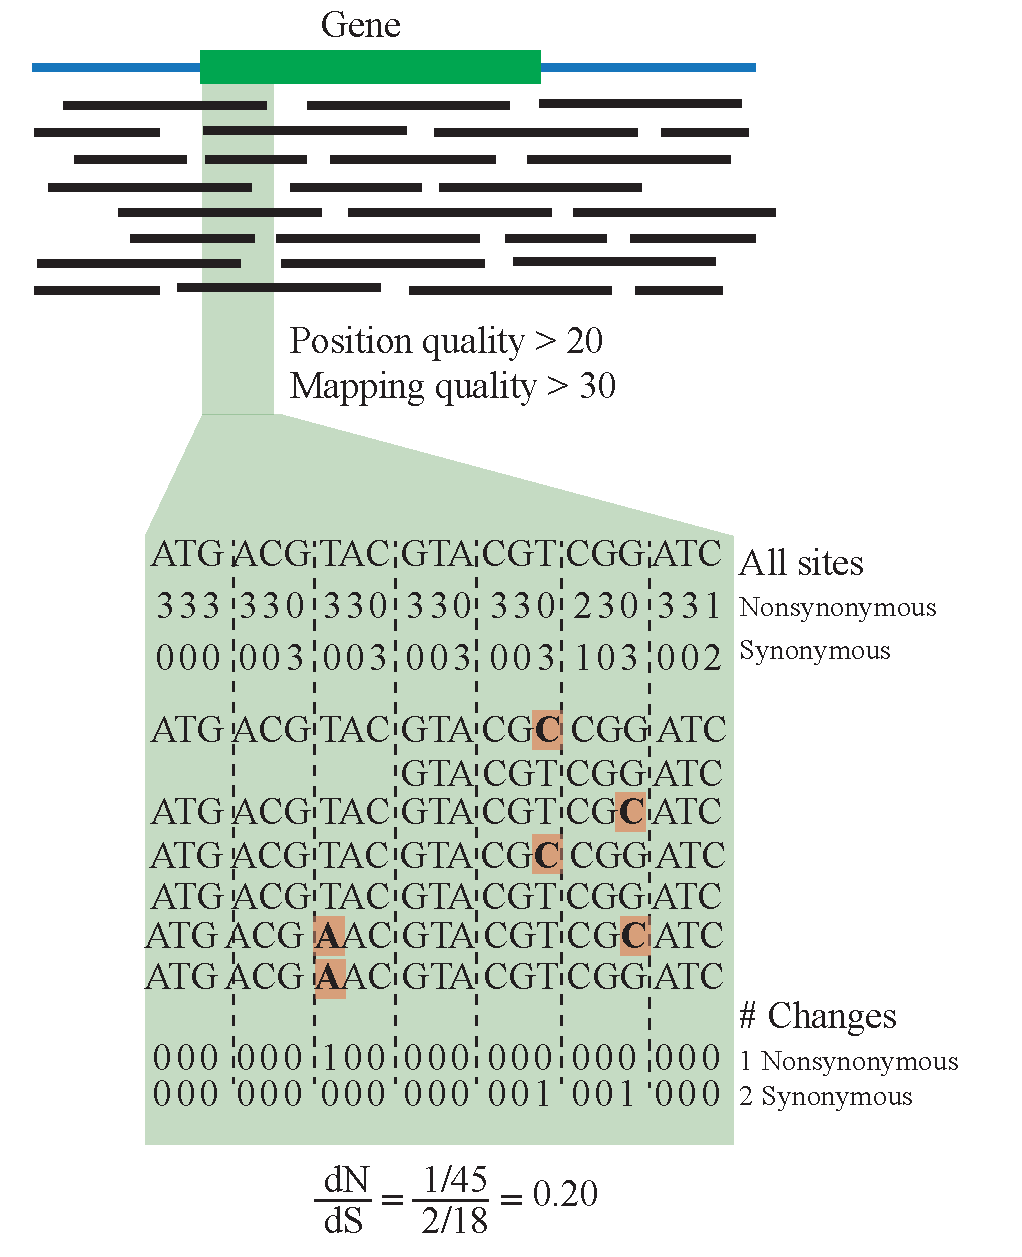
\includegraphics[width=\textwidth]{Chapter5/Figures/MappingStrategy.pdf}
  \caption{Overview of the strategy used to quantify the SNPs differences on each gene, and calculate the ratio of non-synonymous to synonymous substitutions (pN/pS) on each of the reference genome. Figure based on \cite{Tai:2011jo}.}
  \label{MappingStrategy}
\end{figure}

%Table Genes positive selection
\begin{table}[hbt]
  \caption{Count of Genes under positive selection}
  \begin{tabularx}{\textwidth}{L{2.2cm}R{2cm}R{3cm}R{3.2cm}R{2cm}}
  \hline
    \textbf{Genome} & \textbf{CDS} & \textbf{January} & \textbf{August} & \textbf{Unique (Jan/Aug)} \\
    \hline
     \textit{J07HWQ1} & 3,584 & 568 (15.9) & 570 (15.9) & 4/6 \\
     \textit{J07HWQ2} & 3,856 & 565 (14.7) & 561 (14.6) & 6/2 \\
     \textit{J07HQX50} & 2,872 & 406 (14.1) & 405 (14.1) & 3/2 \\
     \textit{J07AB56} & 1,411 & 244 (17.3) & 236 (16.7) & 72/64 \\
     \textit{J07AB43} & 1,678 & 274 (16.3) & 281 (16.8) & 35/43 \\
     \textit{J07HN4} & 3,230 & 428 (13.3) & 427 (13.2) & 5/4 \\
     \textit{J07HN6} & 2,914 & 220 (7.6) & 218 (7.5) & 23/21 \\
     \textit{J07HX64} & 3049 & 603 (19.8) & 603 (19.8) & 3/3 \\
     \textit{J07HX5} & 2,139 & 374 (17.5) & 374 (17.5) & 2/2 \\
     \textit{J07HB67} & 2,847 & 494 (17.4) & 493 (17.3) & 60/59 \\
     \textit{J07HR59} & 1,841 & 145 (7.9) & 155 (8.4) & 3/13 \\
     \textit{A07HB70} & 2,514 & 479 (19.1) & 479 (19.1) & 6/6 \\
     \textit{A07HR67} & 2,891 & 507 (17.4) & 511 (17.7) & 0/4 \\
     \textit{A07HN63} & 2,507 & 212 (8.5) & 240 (9.6) & 9/37 \\
     \textit{A07HR60} & 2,861 & 375 (13.1) & 381 (13.3) & 10/16 \\
     \textit{G22} & 3,525 & 5 (0.14) & 5 (0.14) & 1/1 \\
     \textit{J07SB} & 1,641 & 290 (17.7) & 287 (17.5) & 6/3 \\     
  \end{tabularx}
  \label{PSgenes}
\end{table}

%Figure COG pNpS average
\begin{figure}[!hbtp]
  \centering
  \includegraphics[width=0.7\textwidth,height=\textheight,keepaspectratio]{Chapter5/Figures/Scatter_Genomes_pNpS.pdf}
  \caption{}
  \label{Genome_comp_pNpS}
\end{figure}


%Figure COG pNpS average
\begin{figure}[!hbtp]
  \centering
  \includegraphics[width=\textwidth,height=\textheight,keepaspectratio]{Chapter5/Figures/COG_Average_pNpS.pdf}
  \caption{}
  \label{COG_pNpS_avg}
\end{figure}

\todo{comments about gene products list}

\clearpage
\section{General Discussion}
Population parameters
Broad picture, not focusing on single organisms
MK tests
Fixation ratios, FST
Effects of HGT
Core genome -> need to focus on single groups
It has been argued previously that many genes occurring at intermediate frequency within genomes are involved in predation evasion by varying surface antigenicity 

Correlation of these data with the viral data from Joane (Emerson 2012), regarding the temporal scale variation on the virla community
We didn't explore phagesin this study


\section{Conclusions}

SNPs and INDELs are about low-level genomic variation. It is also possible to look at structural variants which affect the genome at larger scales. Events like gene duplications, tandem repeats, transposon insertions, inversions, and other chromosomal rearrangements are all important to consider, but this post will leave those issues for another day.

Conclusion

SNPs and INDELs are small differences between genomes. They are important drivers of bacterial evolution, by modifying how or whether genes are transcribed and translated. In my next post I will introduce my new tool Snippy for discovering these differences efficiently.

\section{Acknowledgments}
I would like to thank Sheila Podell for discussions on the analysis and ideas for this Chapter. Also, funding from Fulbright-Conicyt and NSF XXXX is acknowledged, and to Amazon Web Services for an education grant that allowed the use of the EC2 infrastructure.


\todo{Print and check font size}
%Figures pn/ps along genome
\begin{figure}[p]
  \centering
  \includegraphics[width=\textwidth,height=\textheight,keepaspectratio]{Chapter5/Figures/pn_ps_plots/J07HWQ1_pNpS_density.pdf}
  \caption{}
  \label{J07HWQ1_pNpS}
\end{figure}

\begin{figure}[p]
  \centering
  \includegraphics[width=\textwidth,height=\textheight,keepaspectratio]{Chapter5/Figures/pn_ps_plots/J07HWQ2_pNpS_density.pdf}
  \caption{}
  \label{J07HWQ2_pNpS}
\end{figure}

%%%%%%%%%%%%%%%%%%%%%%%


%\todo{Modify reference SNPs section}
%\subsection{Genome information and reference SNPs}
%To generate a list of reference SNPs,  11 archaeal genomes obtained from the assembly of the metagenomic samples were analyzed. The results (Table \ref{GenomeTable}), shows the total number of SNPs identified in each of the genomes. Although the low depth of the analysis does not allow to make any assumptions about the levels of genetic heterogeneity present on each population, still can provide a valid picture that can be contrasted with the Illumina data. Figure \ref{ReferenceSNPsType}, shows a comparison of the location and type of variation found among the genomes. Most of the identified polymorphisms are synonymous, meaning that they do not produce any changes in the amino acid sequence. Comparing among the populations, most of the polymorphisms fall into coding regions, with some extreme cases such as in \textit{Nanosalina} sp. J07AB43 and \textit{Nanosalinarum} sp. J07AB56, where only 5\% and 8\%, respectively, of the polymorpshism are found in intergenic regions. This reflects the streamlined nature of these genomes, and their reduced intergenic space \cite{Narasingarao:2012kp}. An interesting situation occurs in the case of \textit{Nanosalina} sp. J07AB43, which has a high number of polymorphisms classified as other (mostly frameshifts), close to a 51\%. This could be either result from assembly problems, or a reflection on the true genetic variability that is present in this population, but a higher level of resolution is needed to resolve this question.
%
%By looking at the annotation of each gene, we can begin to explore the possible functional effects of the found SNPs on each microbial population (Figure \ref{COG_TotalSNPs}). The averages values for each functional classification (Cellular Processes and Signaling: 19.1\%, Information Storage and Processing: 22.6\%, Metabolism: 39.9\% and Poorly characterized: 18.4\%), shows a higher percentage of SNPs (in average) in the metabolic functions. This can easily be explained by the larger number of genes that fall in this category. Even with this in mind, J07HQX50 shows a higher percentage of SNPs associated in the Cellular Processes and Signaling category, while J07AB43 and J07AB56 (members of the \textit{Nanohaloarchaea}) have a higher number of polymorphic sites in genes in the Information Storage and Processing and the Metabolic categories.
%
%Another important way to characterize the effects of the SNPs on each genomes is to look at the non-synonymous substitutions that are occurring across the genome, because the effect of this polymorphisms is to modify the resulting amino acid in the protein. The averages for each functional classification (Cellular Processes and Signaling: 18.1\%, Information Storage and Processing: 23.1\%, Metabolism: 38.5\% and Poorly characterized: 20.13\%), shows very similar values to the total count of SNPs (\ref{COG_NonSynSNPs}). Although the number of total and non-synonymous SNPs found in this part of the analysis is low to draw any conclusions about the effect on the overall microbial population, we observe that in the case of J07HR59 there are no non-synonymous polymorphisms associated with Cellular Processes and Signaling, while most fall in the Information category.
%
%To look more in detail at the effect of these non-synonymous SNPs, we can look more in detail at the functional classifications provided by COG. In the Cellular Processes and Signaling group, we can observe differences for the microbial populations (Figure \ref{ReferenceSNPs_NS_CellularProc}), which could be related to the low coverage observed for this reference SNPs, in particular in the case of J07HQX50, which has most of its SNPs associated with signal transduction mechanisms. Overall, the classification of these non-synonymous SNPs, shows that the majority falls in categories such as cell wall/membrane/envelope biogenesis, post-translational modifications and signal transduction mechanisms. These are functions that are related to the interaction of the organisms with the environments, such as phage infection and resistance mechanisms (REF), transporters (REF) and overall functions where it could be expected that changes in the amino acid sequences could be beneficial for the persistence of the microbial population in the environment. A similar situation can be observed in the case of the Information Storage and Processing category (Figure \ref{ReferenceSNPs_NS_Information}), where the more abundant in functions such as translation, ribosomal structure and biogenesis, and in proteins classified in the replication, recombination and repair group. Later in this chapter, we will explore the environmental adaptations of each microbial population, by using a deep-sequencing approach.
%
%In the case of functions that are part of the Metabolism group in the COG classification (Figure \ref{ReferenceSNPs_NS_Metabolism}), the trend is not as clear as in the other groups. The only two exceptions are J07HQX50 that has most of its polymorphisms associated with the inorganic ion transport and metabolism category, and J07HR59 that has most polymorphisms in the nucleotide transport and metabolism category. 
%
%Overall, this preliminary overview provides a set of expectetions on further analysis on the genetic heterogeneity of some of the microbial populaitons present in the Lake Tyrrell habitat. More important, by deconstructing the assembly of the Sanger reads, we can obtain a set of reference SNPs, which can be used for further population studies. This becomes very important consdiering that none of the organisms that were reocvered from the metagenoms is in culture, so targeting their genomes directly for SNP validation is not feasible, and other proxies need to be used. This dataset will be used for validation of the results of the mapping and variation detection in the following sections of this chapter.
%
%%TABLES
%
%\begin{table}[!htdp]
%\caption{Genome and reference SNPs}
%\begin{center}
%\resizebox{\textwidth}{!}{%
%\begin{tabularx}{\textwidth}{lp{2cm}p{2cm}p{3cm}}
%\hline
%%\textbf{Genome} & \textbf{Scaffold (JGI ID)} & \textbf{Length} & \textbf{SNPs} & \textbf{Change rate} \\
%\textbf{Genome}  & \textbf{Length} & \textbf{SNPs} & \textbf{Change rate} \\
%
%\hline \hline
%\multirow{2}{*}{\textit{Halonotius} sp. J07HN4} & 547,037 & 963 & 568\\
%& 2,341,623 & 7,985 & 293 \\
%\hline
%
%\multirow{6}{*}{\textit{Halonotius} sp. J07HN6} & 61,036 & 603 & 101 \\
% & 89,290 & 558 & 160 \\
% & 185,112 & 1,482 & 124 \\
% & 424,200 & 2,761 & 153 \\
% & 873,166 & 6,463 & 135 \\
%& 896,196 & 5,455 & 164 \\
%\hline
%
%uncultured archaeon sp. J07HX64 & 2,982,938 & 5,468 & 545 \\
%\hline
%\multirow{3}{*}{\textit{Halobaculum} sp. J07HB67} & 110,024 & 62 & 1,744 \\
%& 254,249 & 145 & 1,753 \\
%& 2,285,274 & 2,855 & 800 \\
%\hline
%
%\multirow{2}{*}{\textit{Haloquadratum} sp. J07HQX50} & 1,543,888 & 28 & 55,138 \\
%& 1,476,021 & 131 & 11,267 \\
%\hline
%
%\multirow{4}{*}{\textit{Halorubrum} sp. J07HR59} & 72,446 & 1 & 72,466 \\
%& 49,857 & 29 & 1,719 \\
%& 184,023 & 7 & 26,289 \\
%& 1,672,266 & 255 & 6,557 \\
%\hline
%
%\textit{Haloquadratum walsbyi} J07HQW1 & 3,475,501 & 24,743 & 140 \\
%\hline
%
%\textit{Haloquadratum walsbyi} J07HQW2 & 3,594,539 & 13,897 & 258 \\
%\hline
%
%uncultured archaeon J07HX5 & 2,040,945 & 2,047 & 997 \\
%\hline
%
%\multirow{7}{*}{\textit{Nanosalina} sp. J07AB43} & 54,503 & 295 & 184 \\
%& 111,825 & 1,037 & 107 \\
%& 65,032 & 876 & 74 \\
%& 32,088 & 304 & 105 \\
%& 112,863 & 2,296 & 49 \\
%& 52,428 & 1,288 & 40 \\
%& 798,418 & 11,578 & 68 \\
%\hline
%
%\multirow{3}{*}{\textit{Nanosalinarum} sp. J07AB56} & 195,424 & 1,540 & 127 \\
%& 60,285 & 196 & 307 \\
%& 959,093 & 6,837 & 140 \\
%\hline
%
%
%\end{tabularx}
%}
%\end{center}
%\label{GenomeTable}
%\end{table}
%
%
%%FIGURES
%
%\begin{figure}[!htbp]
%	\centering
%	\includegraphics[width=\textwidth]{Chapter5/Figures/ReferenceSNPtypes.pdf}
%	\caption{Classification of the reference SNPs, by type.}
%	\label{ReferenceSNPsType}
%\end{figure}
%
%%FIGURE
%\begin{figure}[!htbp]
%	\centering
%	\subfloat[Total SNPs \label{COG_TotalSNPs}]{%
%		\includegraphics[width=\textwidth]{Chapter5/Figures/ReferenceSNPs_COGsTotal.pdf}
%	}
%	\hfill
%	\subfloat[Non-synonymous SNPs\label{COG_NonSynSNPs}]{%
%		\includegraphics[width=\textwidth]{Chapter5/Figures/ReferenceSNPs_COGs_NS.pdf}
%	}		
%	\caption{Comparison between the total number and the non-synonymous SNPs found in each genome, associated to functional categories from the COG classification }
%	\label{ReferenceSNPs_COGsSummary}
%\end{figure}
%
%%FIGURE
%
%\begin{figure}[!htbp]
%	\centering
%	\includegraphics[width=\textwidth]{Chapter5/Figures/ReferenceSNPs_NonSyn_CellularProc.pdf}
%	\caption{Count of non-synonymous SNPs found in COGs categories from the Cellular Processes and Signaling group}
%	\label{ReferenceSNPs_NS_CellularProc}
%\end{figure}
%
%\begin{figure}[!htbp]
%	\centering
%	\includegraphics[width=\textwidth]{Chapter5/Figures/ReferenceSNPs_NonSyn_Information.pdf}
%	\caption{Count of non-synonymous SNPs found in COGs categories from the Information Storage and Processing group}
%	\label{ReferenceSNPs_NS_Information}
%\end{figure}
%
%\begin{figure}[!htbp]
%	\centering
%	\includegraphics[width=\textwidth]{Chapter5/Figures/ReferenceSNPs_NonSyn_Metabolism.pdf}
%	\caption{Count of non-synonymous SNPs found in COGs categories from the Metabolism group}
%	\label{ReferenceSNPs_NS_Metabolism}
%\end{figure}
%
%
%

%\subsection{Selection analysis of the reference SNPs}
%- Genes found under positive selection
%- Functional differences of the genes under positive selection
%- Categories, etc

%
%
%Comparison between assembly and read mapping
%
%The comparison between the number of reads used in the assembly of the archaeal populations, versus mapping the reads back to these genomes, indicates that only a low percentage of the reads were not recovered by mapping (XX\%) (Figure X). In addition, mapping of the reads allows the recovery of reads that were not incorporated into the assemblies.
%
%Even when the number the depth of coverage is increase when the reads are mapped back to the reference genomes (Table X), the overall distribution of depths along the genome shows a similar trend (Figure X), indicating that even with that more reads are recruited (increasing the depth of coverage and posiblly the number of SNPS presents compared to an assembly-based analysis), we are not overrepreseting areas of the genome.
%
%We observed differences when looking at the coverage of individual genes, where a small percentage in each genome (XX, Table X) showed less coverage than expected. Neverhelss, this is only a small fraction of the total number of genes present (Figure X).
%
%Look at the gene with transport, secretory or motilify functions in detail. Look a the dN/dS ratiosn in a sliding window (201 bp?)
%
%For hypothetica proteins, look at SCOP classification
%


%
%\begin{figure}[htbp]
%	\centering
%	*
%	\caption{Analysis pipeline workflow}
%	\label{WorkflowAnalysisSNPs}
%\end{figure}
%
%
%\begin{figure}[htbp]
%	\centering
%	*
%	\caption{Mapped reads per genome}
%	\label{ReadMappingGenomes}
%\end{figure}
%
%\begin{figure}[htbp]
%	\centering
%	*
%	\caption{Depth of coverage for each genome}
%	\label{DepthCoverageGenomes}
%\end{figure}
%
%\begin{figure}[htbp]
%	\centering
%	*
%	\caption{SNPs in COGs}
%	\label{COGsSNPs}
%\end{figure}
%
%\begin{figure}[htbp]
%	\centering
%	*
%	\caption{Transition transversion rates}
%	\label{TTrates}
%\end{figure}
%
%\begin{figure}[htbp]
%	\centering
%	*
%	\caption{Network diagram SNPs}
%	\label{NetworkSNPs}
%\end{figure}
%
%\begin{figure}[htbp]
%	\centering
%	*
%	\caption{Map of SNPs in contigs}
%	\label{SNPsContigMap}
%\end{figure}
%
%\begin{figure}[htbp]
%	\centering
%	*
%	\caption{SNP rarefaction curve per population}
%	\label{SNPsRarefaction}
%\end{figure}
%
%\begin{figure}[htbp]
%	\centering
%	*
%	\caption{Calculation of pN/pS ratios}
%	\label{pNpS_diagram}
%\end{figure}
%
%\begin{figure}[htbp]
%	\centering
%	*
%	\caption{Histogram of dN/dS ratios}
%	\label{pNpS_hist}
%\end{figure}



%\bibliographystyle{abbrv}
%\bibliography{CompleteLibrary}